\subsubsection{Controller}
\label{sec:Controller}
	\begin{wrapfigure}{r}{0.45\textwidth}
		\centering
		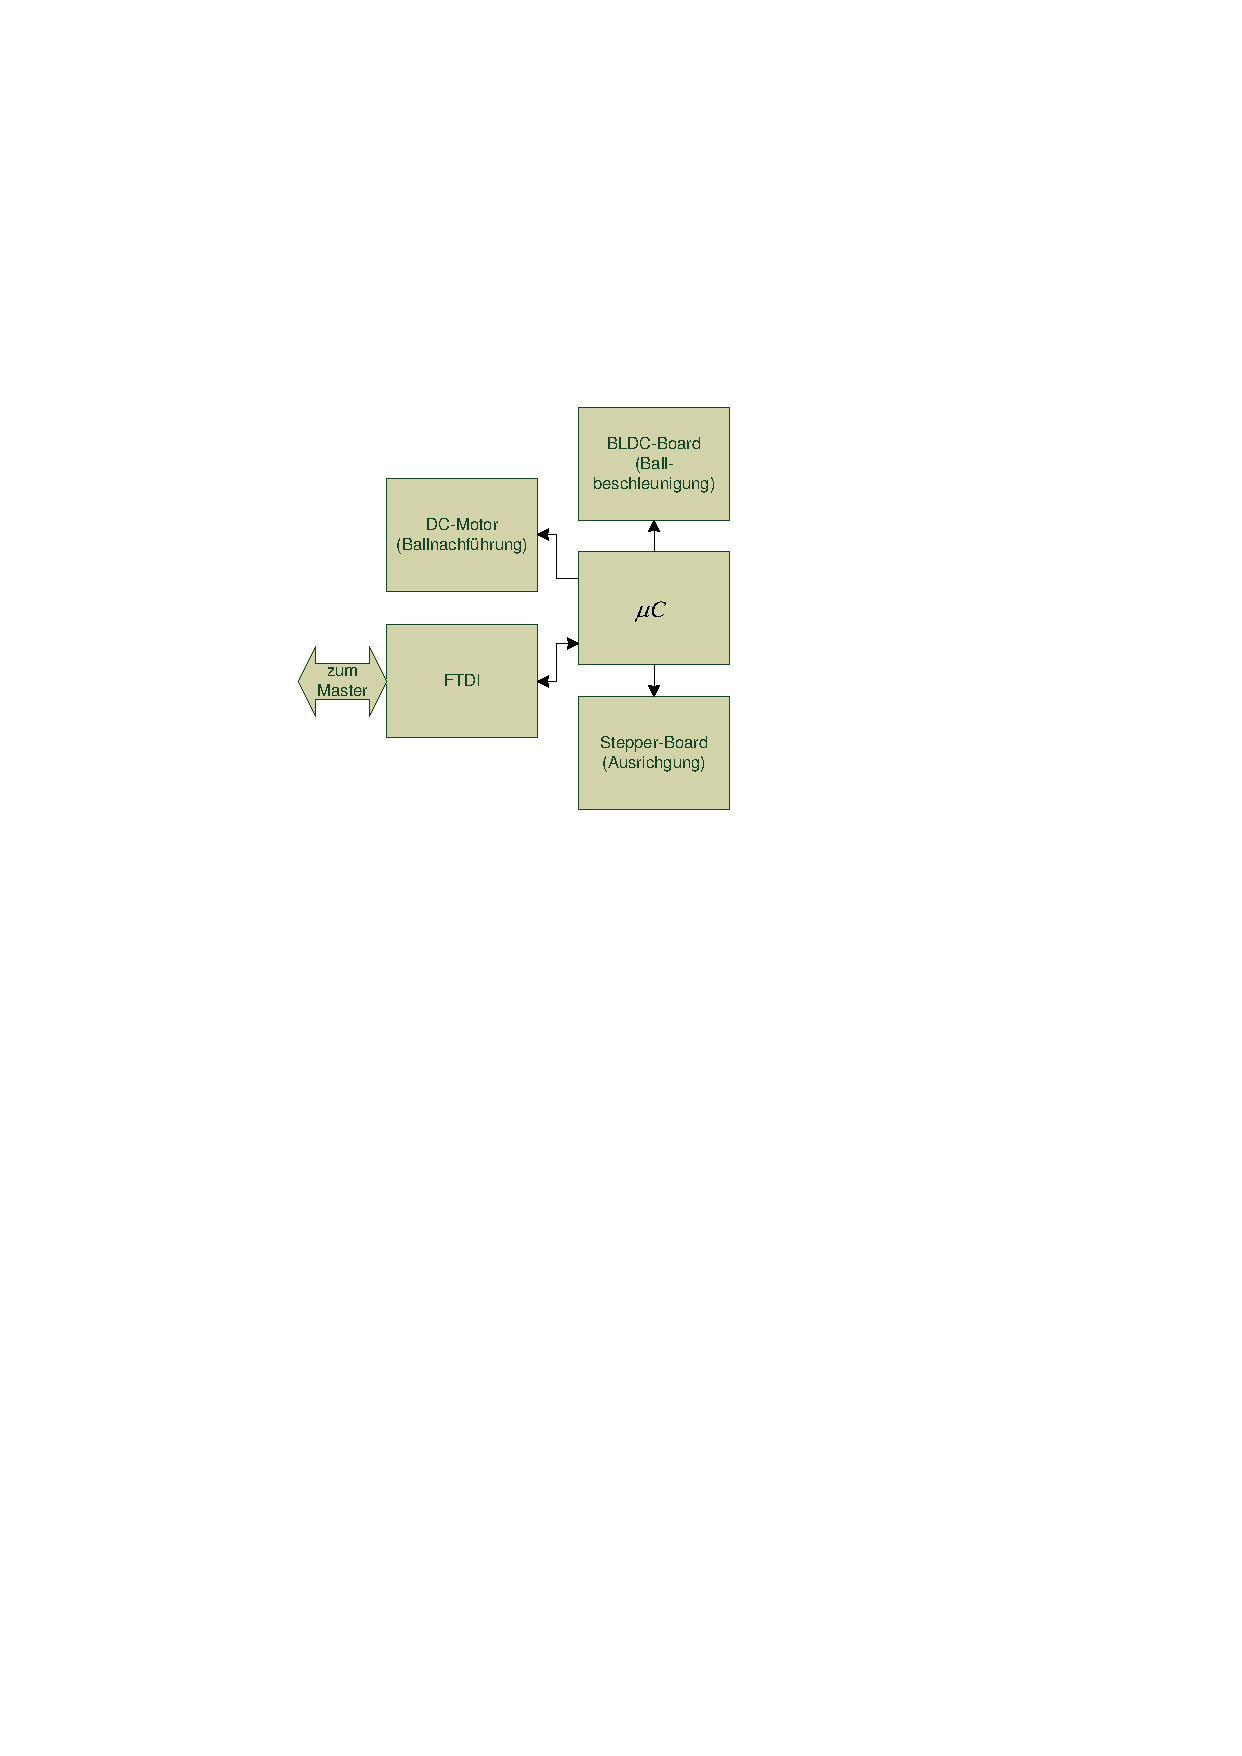
\includegraphics[width=0.44\textwidth,clip,trim= 50mm 16cm 86mm 6.8cm]
			{Enddokumentation/Loesungskonzept/Bilder/Blockschaltbild_Controller.pdf}
		\caption{Blockschaltbild der Controller-Hardware}
		\label{fig:Blockschaltbild_Controller}
	\end{wrapfigure}
	Die Controller-Hardware steuert die Motoren der Ballzuführung, der Stepper für die 
	Ausrichtung der Abwurfeinheit und die Motoren zur Beschleunigung der Bälle. Sobald 
	der Controller das Startsignal vom Smartphone erhält, wird dieser den Motor der 
	Schwungräder aktivieren und auf Nenndrehzahl drehen lassen. Weiter erhält der 
	Controller vom Master die Angabe, in welchem Winkel sich der Korb zum Gerät befindet. 
	Anhand dieser werden die benötigten Schritte berechnet und die resultierenden Befehle 
	an die Motorsteuerung werden abgesetzt. Sobald die Abwurfeinheit die richtige Position 
	eingenommen hat, wird die Ballzuführung aktiviert.\\
	\\	
	Die Abbildung \ref{fig:Blockschaltbild_Controller} zeigt auf, wie die Controller-Hardware 
	aufgebaut wird. Die Brushless-Motor- und Stepper-Ansteuerung wird auf separaten Boards 
	realisiert, wobei die Stepper-Hardware durch die PREN-ET-Gruppe (siehe 
	\ref{chap:Fachgruppe Elektrotechnik}) entwickelt und ebenfalls in dieser Gruppe eingesetzt 
	wird. Als Schnittstelle zwischen den Boards und dem Controller wird SPI\footnote{\textbf{S}erial 
	\textbf{P}eripheral \textbf{I}nterface, Dabei handelt es sich um ein synchronen seriellen 
	Datenbus} eingesetzt, da ein Hauptchip der Stepper-Ansteuerung nur über SPI angesprochen 
	werden kann. Die Kommunikation mit dem Smartphone wir über UART\footnote{\textbf{U}niversal 
	\textbf{A}synchronous \textbf{R}eceiver \textbf{T}ransmitter, Dabei handelt es sich um 
	ein asynchrone serielle Schnittstelle} stattfinden, das über den FTDI\footnote{Bezeichnung 
	für einen USB to Serial Chip, FTDI ist der Herstellername}-Chip auf USB emuliert wird. 
	Die Ansteuerung des DC-Motors wird mittels PWM\footnote{\textbf{P}ulse \textbf{W}idth 
	\textbf{M}odulation, Pulsweitenmodulation} realisiert.